\begin{figure}[h]
    \centering
    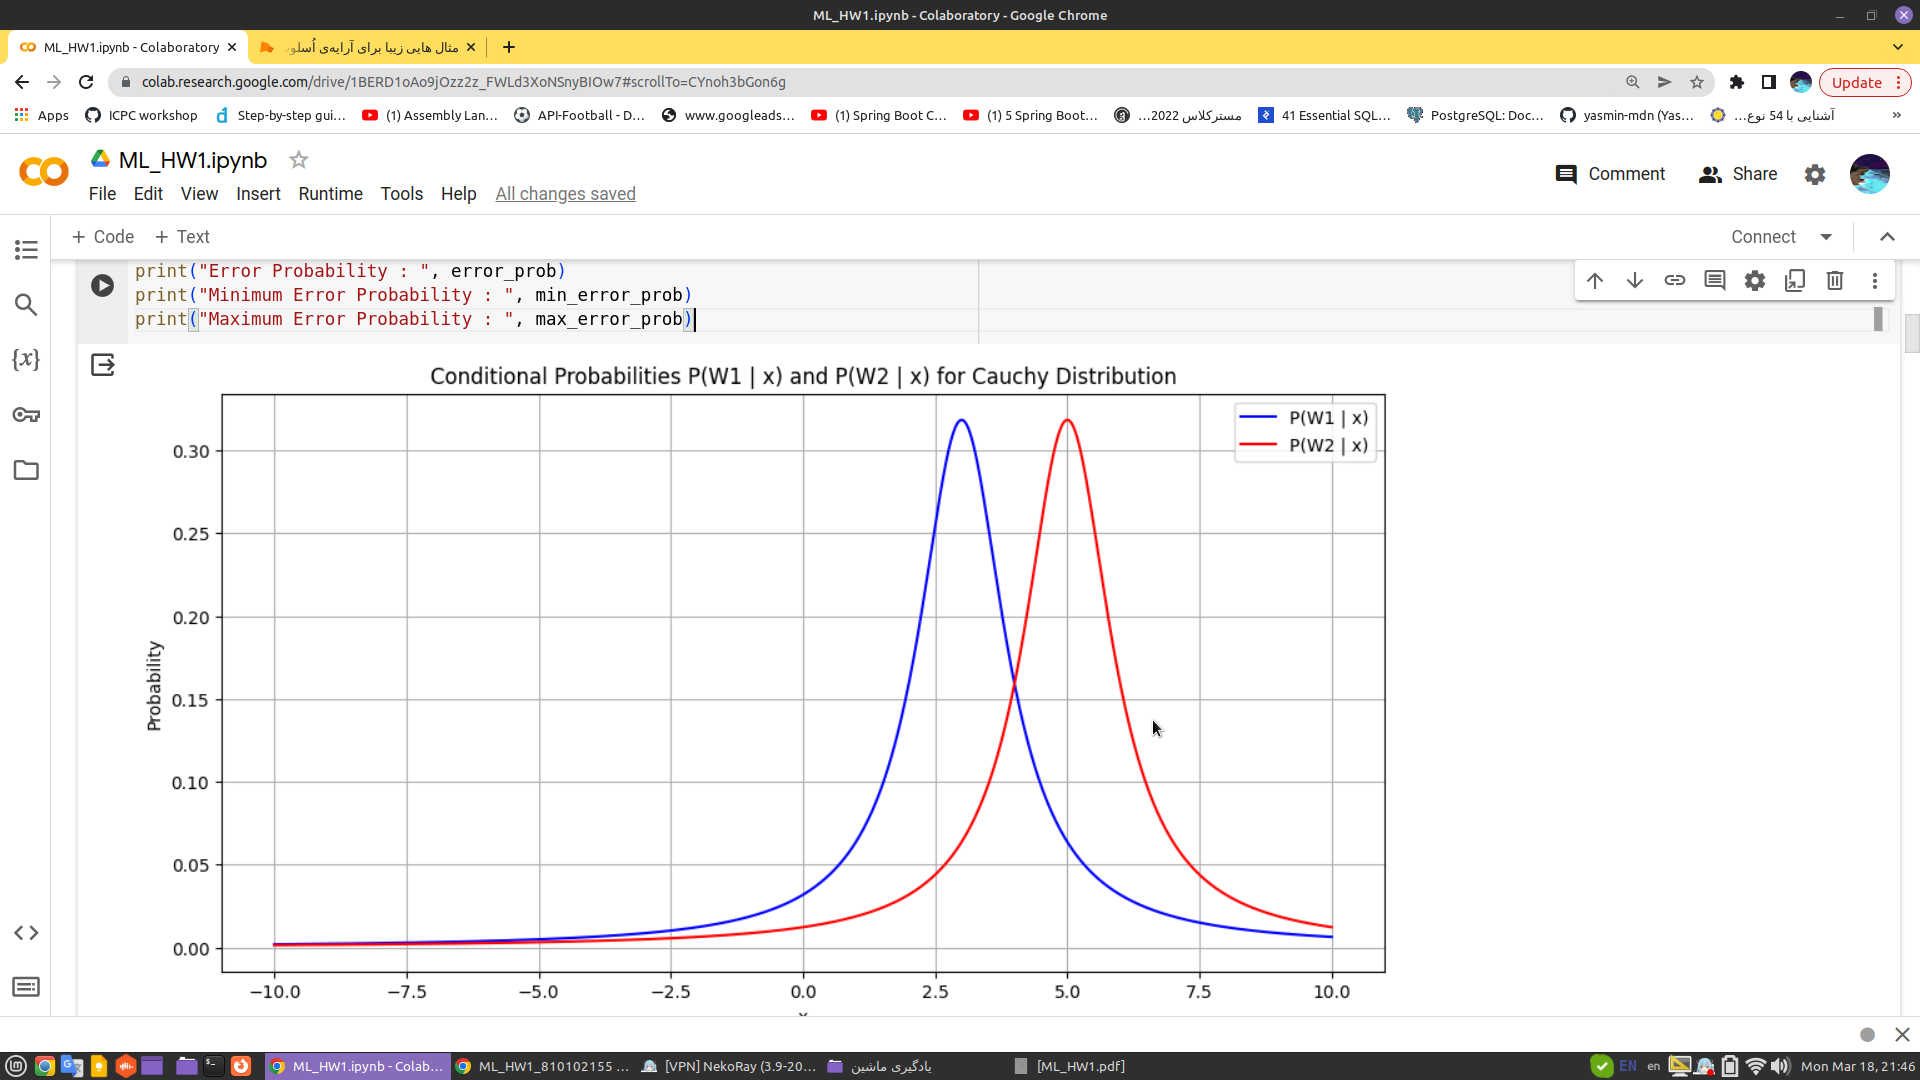
\includegraphics
    [width = 0.8\textwidth]
    {ML1/images/1-A.png}
    \caption{رسم توزیع کوشی برای دو کلاس با مقداردهی هایپرپارامترها}
    \label{fig:enter-label}
\end{figure}

\begin{boxD}
    به منظور رسم شکل فوق می‌بایستی در ابتدا به هایپرپارامترها مقداردهی اولیه کنیم و سپس از تابع احتمال شرطی توزیع کوشی برای رسم استفاده کنیم.

    
     سپس در شکل ۲ همانطور که مشاهده‌می‌فرمایید 
     : 
     \newline
     مرز تصمیم را در میانگین بین میانگین‌های دو توزیع در نظر خواهیم گرفت.

     سپس با محاسبه انتگرال ناحیه خطا خواهیم داشت که مساحت این ناحیه برابر با
     \lr{1.41780}
     می‌باشد.

    سپس در شکل ۳ :
    \newline
     در صورتی که از ماتریس ریسک استفاده کنیم متوجه‌خواهیم‌شد که مرز تصمیم به راست شیفت پیدامی‌کند ، چرا که جریمه به ازای حدس اشتباه کلاس ۱ دو برابر جریمه به ازای حدس اشتباه کلاس ۲ است.

     و 
    \lr{classifier}
     سعی می‌کند که ناحیه خطا را کمینه‌تر کند.

     از شکل ۳ نیز پیدا است که این انتگرال ناحیه خطا برابر با 
     \lr{1.29486} 
     خواهد بود
     .
\end{boxD}

\begin{figure}[h]
    \centering
    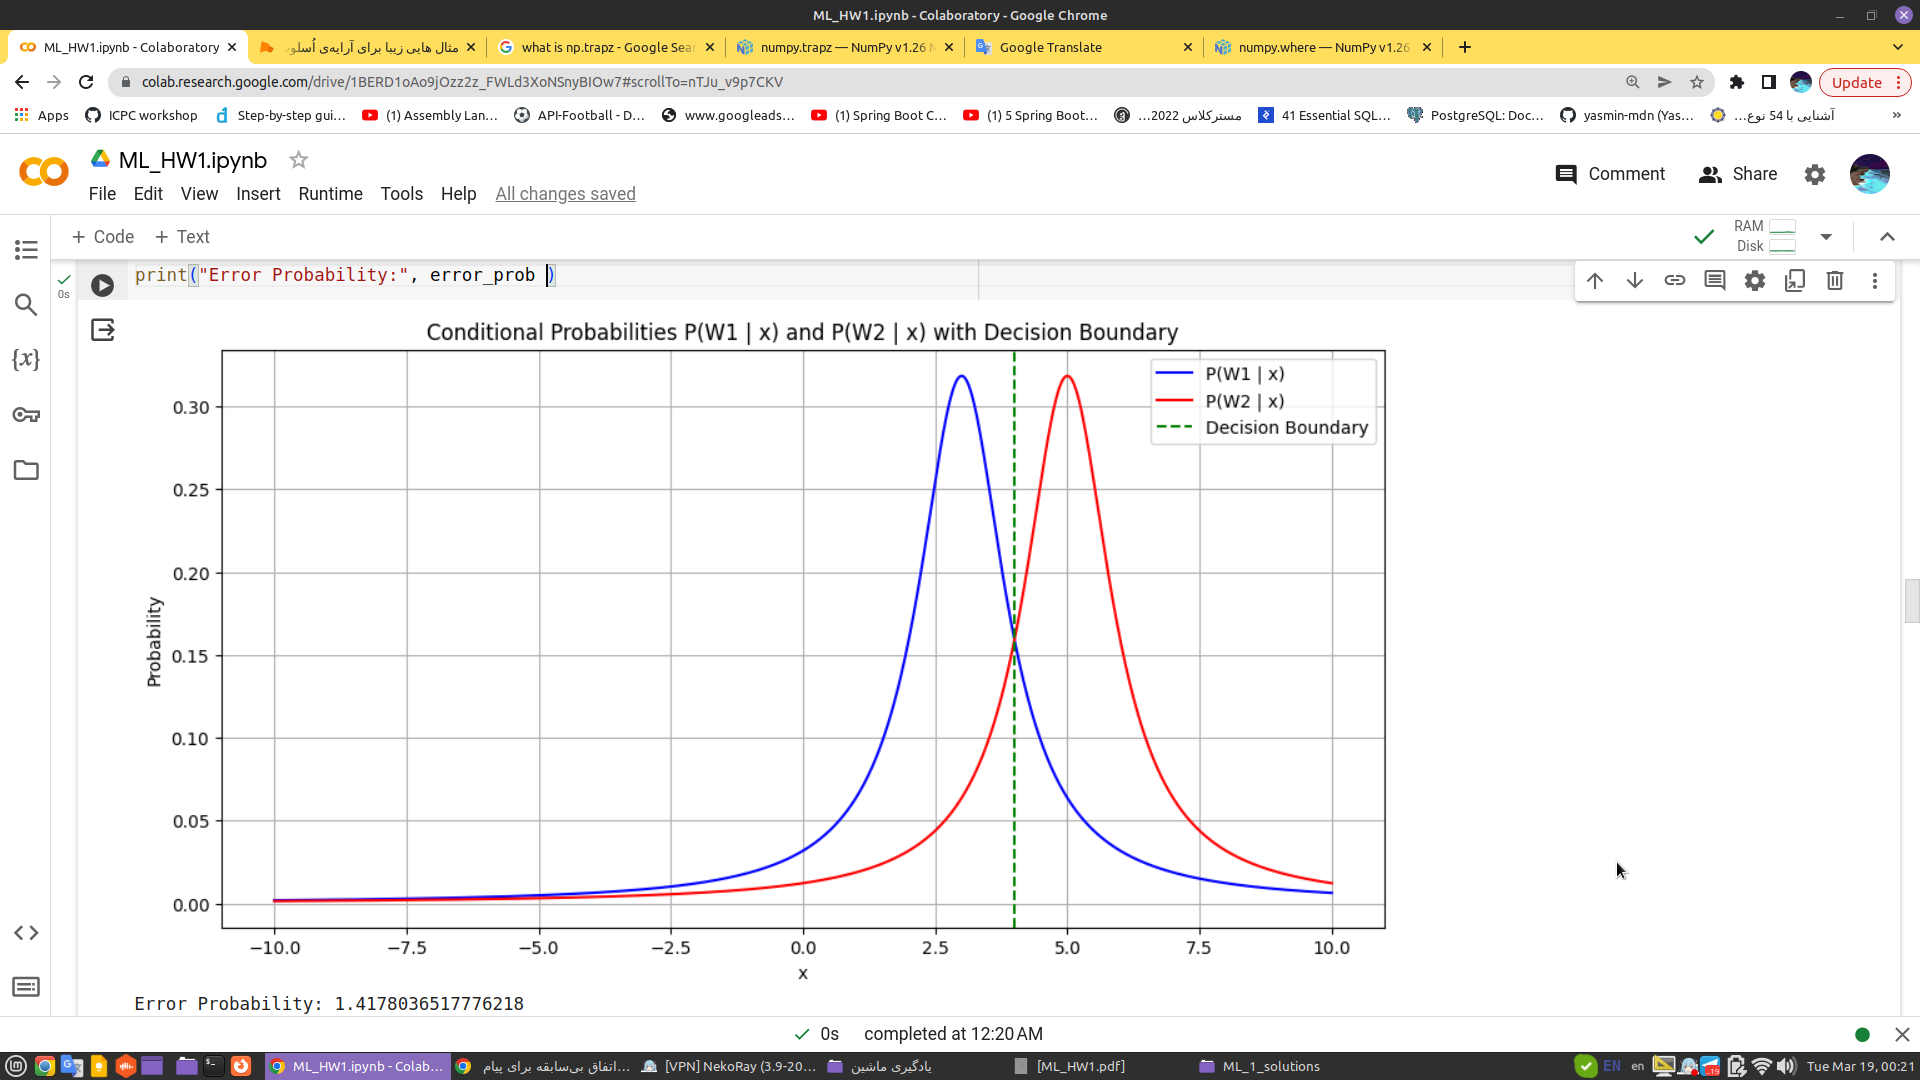
\includegraphics
    [width = 0.8\textwidth]
    {ML1/images/1-T.png}
    \caption{مرز تصمیم برای دو کلاس}
    \label{fig:enter-label}
\end{figure}


\begin{figure}[h]
    \centering
    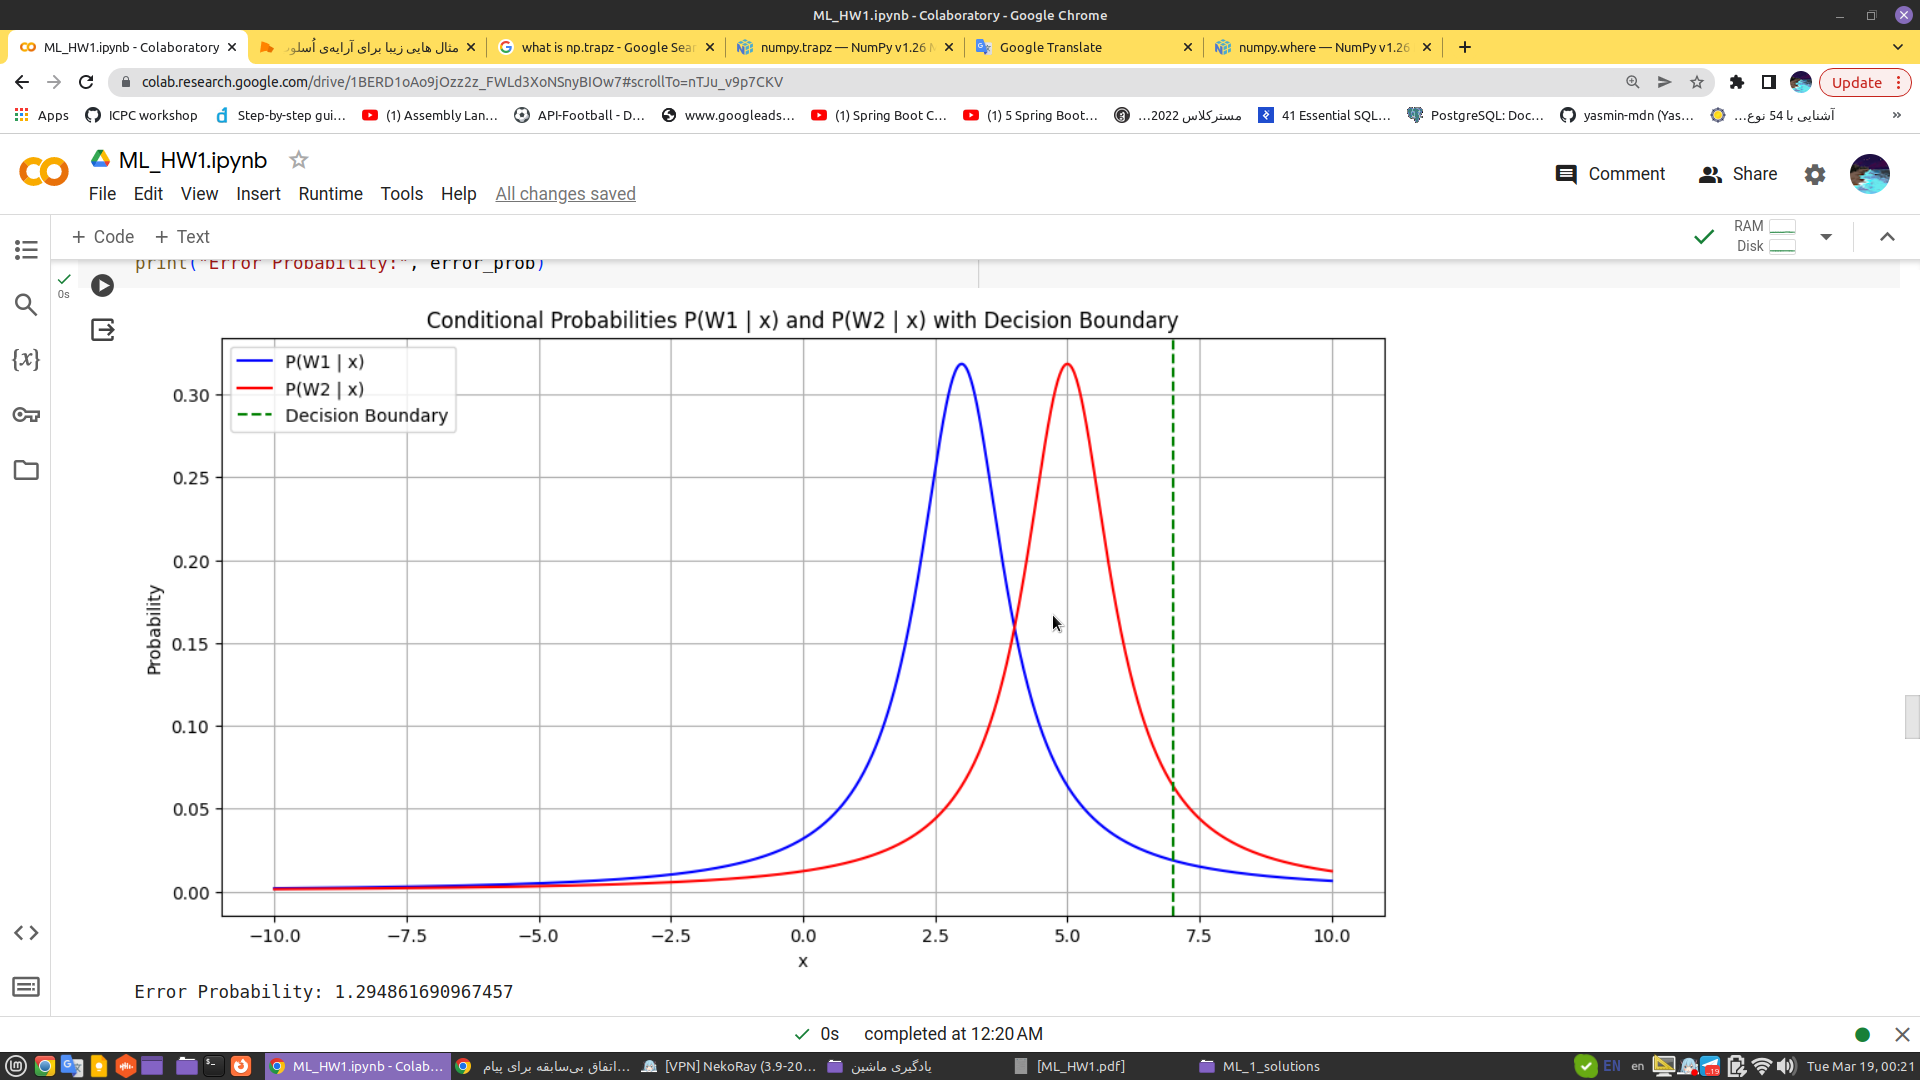
\includegraphics
    [width = 0.8\textwidth]
    {ML1/images/1-S.png}
    \caption{مرز تصمیم برای دو کلاس با توجه به کمینه کردن ماتریس ریسک}
    \label{fig:enter-label}
\end{figure}

\begin{boxA}
    سایر سوالات تشریحی در فایل
    \lr{Razavi ML HW1 810102155}
    پاسخ داده‌شده‌اند.
\end{boxA}


